\chapter{Theoretische Grundlagen}
\label{Kapitel2}

Das folgende Kapitel fokussiert sich darauf, die theoretischen Grundlagen für diese Arbeit zu schaffen. Da es sich nicht um eine Grundlagen Arbeit handelt, werden nur für die Arbeit relevanten Technologien betrachtet und bei tiefergehenden Thematiken auf externe Quellen verwiesen. Vorausgesetzt für diese Arbeit sollte ein grundsätzliches Verständnis über Roboter und Áudiosignale und deren Verarbeitung sein. Im folgenden Abschnitt folgt nun eine Einführung in das Thema ROS.

\section{ROS}

Das \ac{ROS} ist eine umfassende Sammlung von Softwarebibliotheken und Werkzeugen, die speziell für die Robotikentwicklung konzipiert wurde. Es dient als flexible Plattform zur Erstellung von Roboteranwendungen und bietet alles von Treiberintegration bis hin zu modernsten Algorithmen. \ac{ROS} unterstützt eine Vielzahl von Hardwareplattformen und Betriebssystemen, einschließlich Linux, Windows und macOS, und ermöglicht dadurch eine breite Einsatzfähigkeit von Roboterautonomie über Back-End-Management bis hin zu Benutzeroberflächen. Als Open-Source-Projekt ermöglicht \ac{ROS} eine umfassende Zusammenarbeit und Weiterentwicklung durch eine globale Gemeinschaft von Entwicklern und Forschern. Dies fördert nicht nur die Innovation und Verbreitung in verschiedenen Industriezweigen, sondern verkürzt auch die Zeit zur Markteinführung neuer robotergestützter Lösungen \cite{ros_official} \cite{ros_wiki_intro}.

\subsection{Architektur von ROS}

Die Architektur von \ac{ROS} ist als flexibles Framework für die Robotikentwicklung konzipiert. Es handelt sich um ein Meta-Betriebssystem, das Dienste wie Hardwareabstraktion, Steuerung von Niederstufen-Hardware, Implementierung von häufig verwendeten Funktionalitäten, Nachrichtenaustausch zwischen Prozessen und Paketverwaltung bietet.
Zentral für die Architektur von \ac{ROS} ist das Konzept der Knoten (Nodes), die Prozesse darstellen, welche spezifische Aufgaben innerhalb des Gesamtsystems eines Roboters ausführen. Diese Knoten kommunizieren über ein Publish-Subscribe- oder Service-Client-Modell, das den asynchronen und synchronen Nachrichtenaustausch ermöglicht. Knoten können Nachrichten über Themen (Topics) austauschen, Dienste anbieten oder nutzen und auf einen zentralen Parameter-Server zugreifen, um Konfigurationsdaten zu speichern und abzurufen.
Die Modularität ermöglicht es, dass diese Knoten über verschiedene Rechner verteilt und dennoch als einheitliches System betrieben werden können. Diese Verteilbarkeit unterstützt die Skalierung von einfachen bis zu hochkomplexen Robotikanwendungen und fördert die Wiederverwendung von Code innerhalb und zwischen Projekten.


\begin{figure}[H]
    \centering
    \begin{tikzpicture}[
        auto,
        defaultS/.style={
            thick,
            fill=white,
            align=center,
            minimum height=2em,
            draw=black
        },
        boxS/.style={
        	defaultS,
        	rectangle
        },
        ellipseS/.style={
        	defaultS,
        	ellipse
        },
        arrowS/.style={
            -{Latex[length=0.5em]}
        },
        lineS/.style={-},
    ]
    
	\node[ellipseS] (N1) at (0,1) {Node};
	\node[ellipseS] (N2) at (6,1) {Node};
	\node[boxS] (T) at (3,0) {Topic};
	
	\draw[arrowS] (N1) |- node[midway,below]{Veröffentlicht} (T);
	\draw[arrowS] (T) -| node [midway,below] {Aboniert} (N2);
	\draw[arrowS,dotted] (N1) -- node [midway,above] {Service-Aufruf} (N2);
    
    \end{tikzpicture}
    \caption{Einfacher ROS-Graph}
    \label{fig:ros-graph}
\end{figure}


%%%%%%%%%%%%%%%%%%%%%%%%%%%%%%%%%%%%%%%%%%%%%%%%%%%%%%%%%%%%%%%%%%%%%%%%%%%%%%%
\endinput
%%%%%%%%%%%%%%%%%%%%%%%%%%%%%%%%%%%%%%%%%%%%%%%%%%%%%%%%%%%%%%%%%%%%%%%%%%%%%%%


\subsubsection*{Nodes}

Eine Node ist ein Teilnehmer im \ac{ROS} Graphen, der über verschiedene Schnittstelle mit anderen Nodes kommuniziert. Dabei können sich die anderen Nodes im selben, in einem anderen Prozess oder auch auf einem anderen Rechner befinden. Nodes sind typischerweise die Recheneinheiten in einem ROS-Graphen, wobei jede Node eine logische Aufgabe erfüllt.

Nodes können Daten über sogenannte Topics veröffentlichen, um sie an andere Nodes zu senden. Andere Nodes können dann diese Topics abonieren, um Daten von dieser Node zu erhalten. Zusätzlilch können Nodes einen sogenannten Service-Server bereitstellen und für andere Nodes Berechnungen durchführen. Beliebig viele andere Nodes können bei diesem Service-Server Berechnungen in ihrem Namen durchführen lassen. Für länger dauernde Berechnungen können Nodes einen sogenannten Action-Server bereitstellen, der zusätzlich zum Service-Server die Möglichkeit bietet, Berechnungen Abzubrechen und fortlaufende Rückmeldungen über den Stand der Berechnungen zu liefern. Um das verhalten von Nodes während der Laufzeit zu beeinflussen, können diese konfigurierbare Parameter bereitstellen.

Oft stellen Nodes eine komplexe Kombination auws den oben beschriebenen Funktionalitäten da, indem sie zur gleichen Zeit mehrere Topics veröffentlichen und abonieren und verschiedene Services und Actions bereitstellen und von anderen Nodes verwenden.

Verbindungen zwischen Knoten werden automatisch durch die \ac{ROS} zugrundeliegende Middleware hergestellt.

\subsubsection*{Topics}

Topics sind einer der drei Arten von Schnittstellen, die \ac{ROS} bereitstellt und werden für kontinuierliche Datenströme wie Sensorinformationen oder Informationen über den Zustand des Roboters verwendet.

Topics funktionieren nach dem Publish-Subscribe-Prinzip \cite{baldoni2007}.
Hier gibt es zwei Gruppen von Beteiligten, eine die Daten produziert und sendet (Publisher) und eine welche diese empfängt und verarbeitet (Subscriber). Beide Gruppen Nutzen das Topic um miteinander in Kontakt zu treten. Dabei kann es in einem Topic keine oder beliebig viele Publisher geben und ebenso keine oder beliebig viele Subscriber.

\subsubsection*{Services}

Services in \ac{ROS} ermöglichen den Aufruf von Prozeduren in anderen Nodes. Anfragen werden durch eine Node initiiert und durch eine andere Node (den Service-Server) akzeptiert, welcher daraufhin eine Berechnung ausführt. Da die anfragende Node meißtens wartet, bis das Ergebnis eingetroffen ist, werden Services meistens für schnelle Berechnungen verwendet. Services bestehen aus einem Server an den beliebig viele Nodes Anfragen stellen können und werden wie Topics eindeutig durch einen Namen identifiziert. 

\subsubsection*{Actions}

Actions in \ac{ROS} fungieren ähnlich wie Services, sind jedoch auf lang laufende Prozeduren ausgelegt. Wie bei Services sendet eine Node eine Anfrage, hier jedoch an einen Action-Server. Anders als Services können Actions zusätzlich zum Ergebnis fortlaufende Rückmeldungen liefern und bieten die Möglichkeit zum Abbruch durch die anfragende Node. All dies führt jedoch zum einem Mehraufwand beim  erstellen der Verbindung.

\section{Verarbeitung von Audiosignalen}
Nachdem nun im letzten Kapitel Grundlagen über die Arbeit mit Robotern vermittelt wurde soll nun der Fokus auf der Audiosignalverarbeitung liegen. Da es sich hierbei nicht um eine Grundlagen Arbeit handelt wird grundsätzliches Wissen im Bereich Audiosignale und deren Eigenschaften vorausgesetzt. Dieses Kapitel soll einen Überblick darüber schaffen, welche Schritte notwendig sind, um eine Audiosignal erfolgreich zu analysieren und welche Methoden es grundsätzlich für diese Schritte gibt. Eine genauere Analyse der aktuell genutzten Methoden findet in Kapitel \ref{Kapitel3} statt. 

\subsection{Rauschen in Audiosignalen}
Rauschen bezeichnet in der Akustik und Signalverarbeitung jede Art von unerwünschtem Signal, das das Nutzsignal überlagert und dessen Qualität oder Verständlichkeit mindert. Als Maß von Rauschen in Audiosignalen gibt es das Signal-Rausch-Verhältnis (SNR, von englisch Signal-to-Noise Ratio). Es wird üblicherweise in Dezibel (dB) ausgedrückt und gibt an, wie viel höher das Niveau des gewünschten Signals im Vergleich zum Niveau des Rauschens ist. Ein höheres SNR bedeutet, dass das Signal im Verhältnis zum Rauschen stark ist, was allgemein mit einer besseren Qualität des Signals gleichgesetzt wird.


\subsubsection{Rauschquellen}
Nachfolgend sind mögliche Rauschquellen aufgeführt, welche in Audioaufnahmen von robotischen Schleifprozessen auftreten können. Wichtig an dieser Stelle ist zu bemerken, dass nicht alle hier aufgeführten Rauschquellen in diesem speziellen Anwendungsfall als ungewolltes Rauschen aufgefasst werden kann. Vielmehr muss bestimmtes Rauschen analysiert werden um die für diese Arbeit notwendigen Informationen zu beschaffen und eine spätere Klassifizierung vorzunehmen. Welche Rolle die einzelnen Rauschquellen spielen wird zu einem späteren Zeitpunkt bei der Umsetzung der tatsächlichen Rauschfilterung nochmals erläutert.

\begin{enumerate}
    \item \textbf{Mechanisches Rauschen}: Dieses Rauschen entsteht durch die Bewegung mechanischer Komponenten des Roboters und der Schleifausrüstung. Dazu gehören Vibrationen, die durch Unwuchten, Lagerfehler oder die Interaktion des Schleifwerkzeugs mit dem Werkstück entstehen. \cite{xiang2023}
    
    \item \textbf{Elektrisches Rauschen}: Elektrisches Rauschen kann aus der Roboterelektronik oder der Umgebung kommen. Dazu zählen Störungen durch elektromagnetische Felder, die von Motoren, Schaltern und anderen elektronischen Geräten erzeugt werden. \cite{xiang2023}
    
    \item \textbf{Akustisches Rauschen}: Umgebungsgeräusche, wie sie in industriellen Umgebungen üblich sind, können ebenfalls aufgezeichnet werden. Dazu zählen Gespräche, Geräusche anderer Maschinen und Werkzeuge sowie Lärm von Lüftungsanlagen. Zusätzlich können bei Schleifprozessen auch Windgeräusche entstehen, da das Schleifgerät auf eine sehr hohe Drehzahl beschleunigt wird und dadurch Luft umhergewirbelt wird. \cite{xiang2023}
    
    \item \textbf{Interferenzen durch Material und Werkzeug}: Die Art des bearbeiteten Materials und die Beschaffenheit des Schleifwerkzeugs können ebenfalls zu spezifischen Rauschmustern führen. Unterschiedliche Materialien und Werkzeuge erzeugen unterschiedliche Schwingungen und Geräuschpegel. \cite{plos2021}
    
    \item \textbf{Resonanzen im Aufnahmesystem}: Die Komponenten des Audioaufnahmesystems selbst (wie Mikrofone und ihre Befestigungen) können Resonanzen aufweisen, die das aufgezeichnete Signal verzerren. So können auch Resonanzen durch das Audiokabel auftreten, welches beim Schleifprozess Vibrationen ausgesetzt ist.
    
    \item \textbf{Digitales Rauschen}: Bei der Digitalisierung des Audiosignals kann digitales Rauschen auftreten, insbesondere wenn die Hardware nicht hochwertig ist oder falsch kalibriert wurde. Dies kann zu einem Verlust an Klangtreue und Präzision führen. \cite{plos2021}
    
\end{enumerate}

\subsubsection{Filtertechniken}
Da nun ein Überblick darüber geschaffen wurde, was Rauschen ist gilt es nun Möglichkeiten zu finden ungewolltes Rauschen aus der Audiospur zu entfernen. Eine Möglichkeit dies umzusetzen sind Filter.  Es folgt nun eine Übersicht über die gängigsten Filtertypen und ihre allgemeine Anwendung im Kontext der genannten Rauschquellen bei robotischen Schleifprozessen:

\begin{enumerate}

\item \textbf{Tiefpassfilter}
Ein Tiefpassfilter lässt Frequenzen unterhalb einer bestimmten Grenzfrequenz passieren und dämpft Frequenzen oberhalb dieser Grenze.

Anwendung:
\begin{itemize}
    \item Mechanisches Rauschen: Kann effektiv reduziert werden, wenn die Vibrationen zu hochfrequenten Geräuschen führen.
    \item Elektrisches Rauschen: Hochfrequentes Rauschen von elektronischen Komponenten kann gemindert werden.
\end{itemize}

\item \textbf{Hochpassfilter}
Ein Hochpassfilter lässt Frequenzen oberhalb einer bestimmten Grenzfrequenz passieren und dämpft niedrigere Frequenzen.

Anwendung:
\begin{itemize}
    \item Akustisches Rauschen: Tiefere Umgebungsgeräusche, wie das Brummen von Maschinen, können herausgefiltert werden.
\end{itemize}

\item \textbf{Bandpassfilter}
Ein Bandpassfilter lässt nur Frequenzen innerhalb eines bestimmten Bereichs passieren und dämpft Frequenzen außerhalb dieses Bereichs.

Anwendung:
\begin{itemize}
    \item Interferenzen durch Material und Werkzeug: Wenn das Rauschen oder die nützlichen Signale in einem bekannten Frequenzband liegen, kann ein Bandpassfilter eingesetzt werden.
\end{itemize}

\item \textbf{Bandstoppfilter (Notch-Filter)}
Ein Bandstoppfilter, auch als Notch-Filter bekannt, dämpft Frequenzen in einem schmalen Bereich und lässt Frequenzen außerhalb dieses Bereichs passieren.

Anwendung:
\begin{itemize}
    \item Resonanzen im Aufnahmesystem: Spezifische Resonanzfrequenzen, die durch die Aufnahmeausrüstung verursacht werden, können gezielt unterdrückt werden.
\end{itemize}
\end{enumerate}

\subsection{Fourier-Transformation}
Die Fourier-Transformation ist ein grundlegendes Werkzeug bei der Analyse von Audiosignalen. Sie ermöglicht ein Signal aus der Zeitdomäne in die Frequenzdomäne zu transformieren. Das heißt, das Signal wird in seine Frequenzen und die dazugehörigen Amplituden zerlegt. Benannt ist sie nach dem französischen Mathematiker Jean-Baptiste J. Fourier, der im 19. Jahrhundert die Herzfrequenz von Menschen untersuchte und dabei wichtige Grundlagen auf diesem Gebiet entwickelte \cite{Fourier1822}.

Im Wesentlichen zerlegt die Fourier-Transformation ein zeitabhängiges Signal in eine Summe von Sinus- und Kosinusfunktionen unterschiedlicher Frequenzen und Amplituden. 
Diese Bestandteile werden als Frequenzkomponenten des Signals bezeichnet. Das Ergebnis der Fourier-Transformation ist das Frequenzspektrum des ursprünglichen Signals, das angibt, welche Frequenzen im Signal enthalten sind und mit welcher Amplitude diese vertreten sind \cite{Wirsing2020}.

\begin{figure}[H]
    \centering
    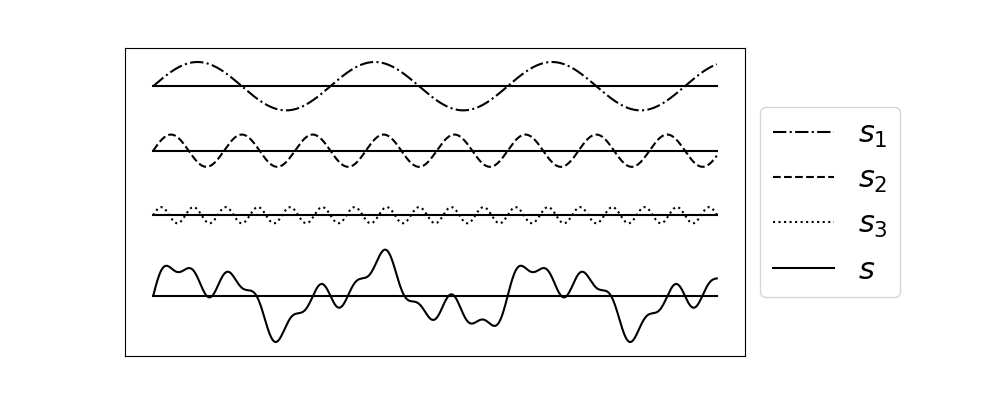
\includegraphics[width=1\linewidth]{images/simple_signal.png}
    \caption[Beispiel Signal \(s\)] {Ein Signal \(s\) zusammengesetzt aus verschiedenen Sinusfunktionen \\ \(s_1 : x \mapsto 1.5 \cdot sin(2x)\), \(s_2 : x \mapsto 1 \cdot sin(5x)\), \(s_3 : x \mapsto 0.5 \cdot sin(11x)\)}
    \label{fig:simple_signal}
\end{figure}

Beispielhaft betrachten wir das Signal \(s\) aus Abbildung \ref{fig:simple_signal}.
Dabei ist das Signal \(s\) die Summe folgender drei Sinusfunktionen:
\begin{align*}
s_1(x) =& 1.5 \cdot sin(2x) \\
s_2(x) =& 1 \cdot sin(5x) \\
s_3(x) =& 0.5 \cdot sin(11x) \\
\end{align*}
Die Sinusfunktionen haben jeweils, unterschiedliche Frequenzen und Amplituden:

\begin{itemize}
    \item \(s_1\) hat eine Frequenz von \(2\) und eine Amplitude von \(1.5\)
    \item \(s_2\) hat eine Frequenz von \(5\) und eine Amplitude von \(1\)
    \item \(s_3\) hat eine Frequenz von \(11\) und eine Amplitude von \(0.5\)
\end{itemize}

\begin{figure}[H]
    \centering
    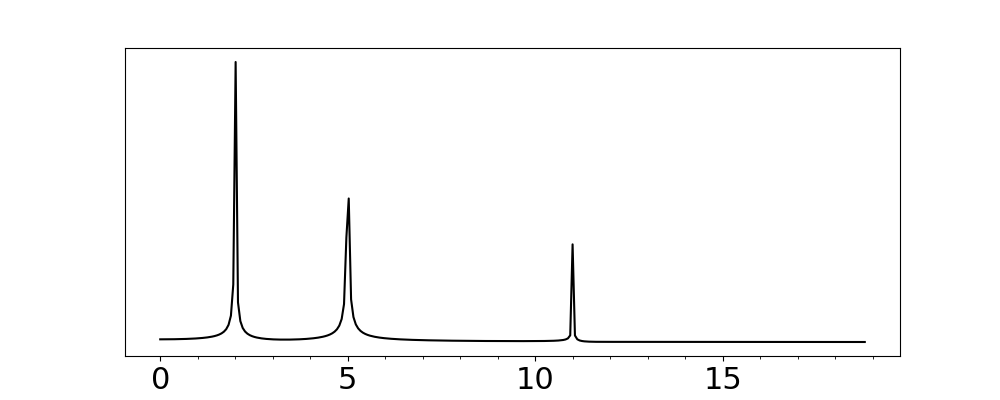
\includegraphics[width=1\linewidth]{images/simple_fft.png}
    \caption[Fourier-Transformation des Signals \(s\)] {Fourier-Transformation des Signals \(s\) aus Abbildung \ref{fig:simple_signal}}
    \label{fig:simple_fft}
\end{figure}

Abbildung \ref{fig:simple_fft} zeigt die Frequenzkomonenten des Signals \(s\) nach der Fourier-Transformation. Auf der x-Achse sind dabei die Frequenzen aufgetragen und auf der y-Achse die Amplituden dieser Frequenzen.
Man erkannt deutlich drei Peaks.
Einen Peak bei einer Frequenz von \(x_1 = 2\) mit einer relativ hohen Ausprägung, einen Peak bei \(x_2 = 5\) mit einer deutlich niedrigeren Ausprägung und einen bei \(x_3 = 11\) mit der niedrigsten Ausprägung.

\subsection{Wavelet} \label{ss:wavelet}

Ein Wavelet ist eine mathematische Funktion, die, wie die oben genannte Fourier-Transformation zur Analyse von Signalen verwendet werden kann. Ein Problem bei der Fourier-Transformation ist jedoch, das die Information über die Zeit verloren geht. So besitzen zum Beispiel ein Audiosignal und dessen Spiegelung exakt das gleiche Frequenzspektrum. \cite{Lee1999}

Im Gegensatz dazu kann man mithilfe einer, Wavelet-Transformation das Signal sowohl in die Zeit- als auch in dessen Frequenzdomänen zerlegen. Dies bedeutet, dass Wavelets Informationen über die Frequenzverteilung eines Signals sowie über die zeitliche Lokalisierung von Ereignissen liefern können.

\begin{figure}[H]
    \centering
    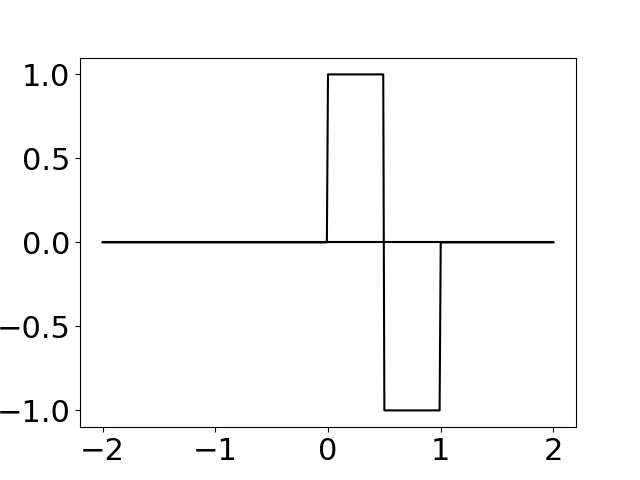
\includegraphics[width=0.5\linewidth]{images/haar.png}
    \caption{Haar-Wavelet}
    \label{fig:haar-wavelet}
\end{figure}

Das Besondere an Wavelets ist, dass sie lokalisiert sind, was bedeutet, dass sie nur in einem begrenzten Bereich des Signals signifikant von null abweichen, im Gegensatz zu den sinusförmigen Funktionen der Fourier-Transformation, die über das gesamte Signal ausgedehnt sind. Dies macht Wavelets besonders nützlich für die Analyse von Signalen mit diskreten Ereignissen oder abrupten Veränderungen, wie zum Beispiel bei der Analyse periodischen Wetterphänomenen \cite{Schulte2019}.

\begin{figure}[H]
    \centering
    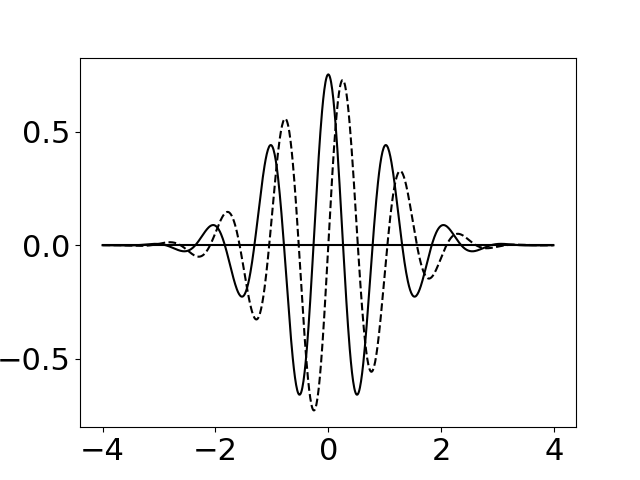
\includegraphics[width=0.5\linewidth]{images/morlet.png}
    \caption{Morlet-Wavelet}
    \label{fig:morlet-wavelet}
\end{figure}

Eine häufig verwendete Wavelet-Funktion ist das Haar-Wavelet (siehe Abbildung \ref{fig:haar-wavelet}):

\begin{equation} \label{eq:haar}
    \psi (t) \; = \; 
    \begin{cases}
        1 \quad &0 \leq \: t \: < \: {1 \over 2} \\
        -1      &{1 \over 2}  \leq \: t \: < \: 1 \\
        0       &\texttt{sonst}
    \end{cases}
\end{equation}

Es ist die einfachste Form des Wavelets. Ein weiteres, häufig verwendetes Wavelet ist das Morlet-Wavelet (siehe Abbildung \ref{fig:morlet-wavelet}):

\begin{equation} \label{eq:morlet}
    \psi (t) \; = \; \pi^{-{1 \over 4}} e^{i\omega_0 t}e^{-{t^2 \, / 2}}
\end{equation}

Wobei \(\omega_0\) (hier \(\omega_0 \; = \; 6\)) die Anzahl der Maxima im Wavelet verändert. \cite{Torrence1998}

%%%%%%%%%%%%%%%%%%%%%%%%%%%%%%%%%%%%%%%%%%%%%%%%%%%%%%%%%%%%%%%%%%%%%%%%%%%%%%%
\endinput
%%%%%%%%%%%%%%%%%%%%%%%%%%%%%%%%%%%%%%%%%%%%%%%%%%%%%%%%%%%%%%%%%%%%%%%%%%%%%%%
